U opent het wachtlijst venster door in het hoofdmenu op de knop ``Wachtlijst'' te klikken. Het wachtlijst venster bestaat uit een aantal knoppen,
	waarmee U de wachtlijst kunt bekijken en manipuleren.
	Op de wachtlijst zelf staan mensen die geopereerd moeten worden,
	maar die nog niet ingepland zijn.\\
\\
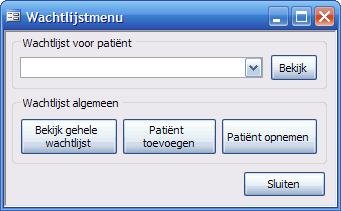
\includegraphics[scale=.7]{wachtlijst1}

\section{Wachtlijst bekijken} \label{sec:wachtlijst bekijken}
	Met de knop ``Bekijk gehele wachtlijst'' krijgt U een lijst met alle mensen op de wachtlijst. Om per pati\"ent deze wachtlijst te bekijken selecteert U in het gebied ``Wachtlijst voor pati\"ent'' een pati\"ent uit het uitrol menu en klikt U vervolgens op de knop ``Bekijken''. Met de twee andere knoppen kunt U pati\"enten aan de wachtlijst toevoegen of op laten nemen.\\

\section{Aan wachtlijst toevoegen} \label{sec:toevoegen}
	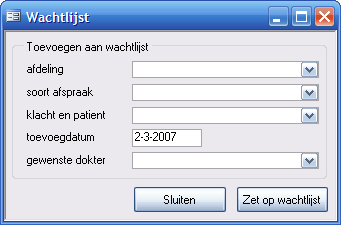
\includegraphics[scale=.6]{wachtlijst2}\\
  \\
	De knop ``Zet op wachtlijst'' opent een venster waarin U een pati\"ent en een klacht selecteert, het gewenste type operatie en de dokter die gaat opereren. Als alles naar wens is ingevuld
	klikt U op de knop ``Zet op wachtlijst''.
	
\section{Van wachtlijst tot opname} \label{sec:opname inplannen}
	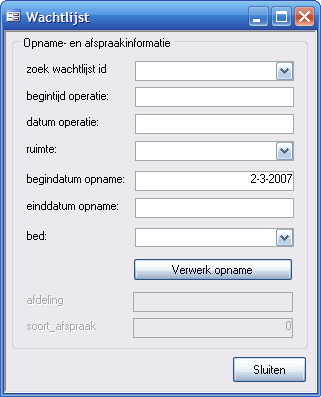
\includegraphics[scale=.6]{wachtlijst3}\\
  \\
	Als er plaats in het ziekenhuis is vrijgekomen kunnen er nieuwe pati\"enten vanaf de wachtlijst worden opgenomen. Met het wachtlijstnummer kunt U makkelijk zoeken naar personen die op de wachtlijst staan. Met de knop ``Verwerk opname'' wordt een pati\"ent van de wachtlijst gehaald en er wordt een opname ingepland \'en een afspraak voor een operatie gemaakt. Dit gaat als volgt: In een nieuw venster krijgt U een rapport te zien waarin U een beter overzicht van de complete wachtlijst krijgt. Ook kunt U informatie invullen over de operatie en de opname van de pati\"ent.

